\section{Robotic arm Kinematic Analysis}


\subsection{Robotic arm, DH parameters \& Forward Kinematics}

The Forward Kinematics problem seeks to specify the way in which the robot's links are connected together. In other wants, we want to specify 
the transformations between every pair of consecutive robot links. It is known that the forward kinematics of a robot can be calculated given only four 
parameters for each link. These parameters are known in robotics as the \textbf{Denavit-Hartenberg} (DH) parameters. Two of these parameters describe the link 
itself and the other two describe the link's relation to the neighboring link.

\begin{itemize}
\item The \textbf{length} $L_i$ of the i-th link is equal to the distance between the axes $z_i$ and $z_{i+1}$
\item The \textbf{twist angle} $α_i$ of the i-th link, is the angle between the axes $z_i$ and $z_{i+1}$
\item The \textbf{rotation angle} $θ_i$ of the link $\left\lbrace i \right\rbrace $ with respect to the $\left\lbrace i-1 \right\rbrace$ link, is the angle 
between the axes $x_{i-1}$ and $x_i$
\item The \textbf{distance} $d_i$ of the link $\left\lbrace i \right\rbrace$ with respect to the $\left\lbrace i-1 \right\rbrace$ link, is the distance 
between the axes $x_{i-1}$ and $x_i$
\end{itemize}

\begin{center}
\begin{figure}[H]
\centering
\includegraphics[height=12cm]{images/iiwa-frames.png}\\
\caption{Joint reference frames of the KUKA iiwa14 robot}
\end{figure}
\end{center}

\begin{center}
\begin{tabular}{ |c|c|c|c|c| } 
\hline
i & $θ_i$ (rad) & $L_{i-1}$ (m) & $d_i$ (m) & $α_{i-1}$ (rad) \\
\hline
1 & $θ_1$ & 0 & 0.36 & 0 \\
2 & $θ_2$ & 0 & 0 & $-π/2$ \\
3 & $θ_3$ & 0 & 0.36 & $π/2$ \\
4 & $θ_4$ & 0 & 0 & $π/2$\\
5 & $θ_5$ & 0 & 0.4 & $-π/2$ \\
6 & $θ_6$ & 0 & 0 & $-π/2$ \\
7 & $θ_7$ & 0 & 0 & $π/2$ \\
\hline
\end{tabular}
\end{center}

Using the DH parameters of the above table, one can calculate the transformation matrix between two consecutive links, and is calculated as the following

\begin{equation}
^{i-1}T_i = 
\begin{bmatrix}
c\theta_i & -s\theta_i & 0 & L_{i-1} \\
s\theta_ica_{i-1} & c\theta_ica_{i-1} & -sa_{i-1} & -sa_{i-1}d_i \\
s\theta_isa_{i-1} & c\theta_isa_{i-1} & ca_{i-1} & ca_{i-1}d_i \\
0 & 0 & 0 & 1\\
\end{bmatrix}
\end{equation}

When all the neighboring transformations are calculated, then one can calculate the total transformation $^{0}T_N$, which represents the position and the 
orientation of the local coordinate system of the end-effector with respect to the global coordinate system of the robot's base. The orientation is the 
upper-left 3x3 matrix and the position is given by the fourth column of the matrix $^{0}T_N$.

\begin{equation}
^{0}T_N = {}^{0}T_1 \cdot {}^{1}T_0 \cdots {}^{N-1}T_N
\end{equation}

All transformations $^{i-1}T_i$ are members of a special set of matrices (Lie Group), called \textbf{Special Euclidean Group}
\[
^{i-1}T_i \in SE(3) = \left\lbrace \begin{bmatrix}
R & \mathbf{p}\\
\mathbf{0} & 1
\end{bmatrix} : R \in SO(3), \mathbf{p} \in \mathbb{R}^{3} \right\rbrace
\]
where $SO(3)$ is another Lie Group called \textbf{Special Orthogonal Group}
\[
SO(3) = \left\lbrace R \in \mathbb{R}^{3 \times 3}: R^{-1}=R^\top, det(R)=1 \right\rbrace
\]

The properties of $SE(3)$ and $SO(3)$ are very useful in all the calculations of various transformations because it can reduce the amount of matrix operations and also speeds up the calculation 
of inverse matrices.

\begin{center}
\begin{figure}[H]
\centering
\includegraphics[width=0.5\textwidth]{images/workspace_sampling_1e3.png}\\
\caption{Approximation of the KUKA iiwa14 workspace, calculated with Forward Kinematics by randomly sampling the value ranges of the joints.}
\end{figure}
\end{center}


\subsection{Inverse Kinematics}

The Inverse Kinematics problem is one of the most important problems a roboticist must solve to design trajectories and control the robot's motion to do useful tasks. The IK problem seeks to find 
those joint values that make the robot's end effector to be at a specific desired position and orientation or equivalently the input to this problem is the desired pose (position and orientation of the end-effector) 
and the output are the solutions for the joints. For a robot of six degrees of freedom, i.e. six actuators that move independently and are positioned in such a way so that their axes are not aligned, the solutions 
to the I.K. problem are typically 8. For robots with more actuators than the 6 degrees of freedom of motion in 3D space (3 for position and 3 for orientation), like the robot of this thesis which has 7 degrees of freedom, 
the I.K. problem has infinite solutions for a given pose, which means that an additional constraint is required to find a specific solution. This extra degree of freedom is very useful in finding kinematic solutions 
that are optimal under some circumstances and are also useful in avoiding \textbf{singularity points} where the robot loses some degrees of freedom.

\subsubsection{Decoupling Technique}

In this section the inverse kinematics problem is solved for only the 6 out of the 7 total degrees of freedom. The third joint is not used in this 
analysis and it's angle is set to zero $θ_3 = 0$ . The rest of the joints form a special kind of kinematic chain that can be solved using the 
decoupling technique. In this technique the Inverse kinematics problem is split to 2 separate subproblems, one for the position and one for the 
orientation of the end-effector. This technique can be applied in this case because the axes of the 3 last joints intersect at the same point and 
they form an Euler wrist. \\

To solve for the joints' angles, the transformation matrix $^0T_7$ of the end-effector with respect to the robot's base is required. Usually the transformation ${}^UT_{tcp}$ is known, which is the pose of Tool's center point (TCP) with respect to the Universal Coordinate Frame $\lbrace U \rbrace$ from which the required $^0T_7$ can be calculated

\begin{equation}
{}^UT_{tcp} = {}^UT_0  \;\;  {}^0T_7  \;\;   {}^7T_{tcp}
\end{equation}

\begin{equation}
{}^0T_7 = {}^UT_0^{-1}  \;\;  {}^UT_{tcp}  \;\;  {}^7T_{tcp}^{-1}
\end{equation}

\begin{equation}
{}^0T_7 = \begin{bmatrix}
R_t & \mathbf{p}_t \\
0 & 1 \\
\end{bmatrix}
\end{equation}

where ${}^UT_0,  \;\;   {}^7T_{tcp}$ are translation transformations by a constant distance and $R_t,  \;\; \mathbf{p}_t$ are the target's orientation 
and position respectively.

\begin{equation}
{}^0\mathbf{p}_5 = {}^0T_4 {}^4\mathbf{p}_5 = \begin{bmatrix} p_x \\ p_y \\ p_z \\ \end{bmatrix}
\end{equation}

\begin{equation}
θ_1 = 
\begin{cases}
atan2 \left( p_y, p_x \right) \\
π - atan2 \left( p_y, p_x \right)
\end{cases}
\end{equation}

\begin{center}
\begin{figure}[H]
\centering
\includegraphics[width=8cm]{images/th2-4-calculation.png}\\
\caption{Calculation of angles $θ_2, θ_4$}
\end{figure}
\end{center}

\begin{equation}
φ = acos \left( \frac{d_3^2 + \Vert{}^1p_{5}\Vert ^2 - d_5^2}{2d_3 \Vert{}^1p_{5}\Vert} \right)
\end{equation}
\begin{equation}
θ_2 = atan2 \left( \sqrt{p_x^2 + p_y^2}, {}^1p_{5z} \right) \pm φ
\end{equation}

\[ c_4 = \frac{ \Vert{}^1p_{5}\Vert ^2 - d_3^2 - d_5^2 }{2d_3d_5} \]
\begin{equation}
θ_4 = atan2 \left( \pm \sqrt{1 - c_4^2}, c_4 \right)
\end{equation}

Once $θ_1,θ_2,θ_3,θ_4$ are known, the orientation matrix of the wrist can be calculated as following
\[
R_{target} = 
\begin{bmatrix}
i_x & j_x & k_x\\
i_y & j_y & k_y\\
i_z & j_z & k_z\\
\end{bmatrix}
\]
\begin{equation}
θ_6 = atan2 \left( \pm \sqrt{1-k_y^2}, k_y \right)
\end{equation}
\[
θ_7 = atan2 \left( -j_y, i_y \right)
\]
\[
θ_5 = atan2 \left( - k_z, k_x \right)
\]

\begin{center}
\begin{figure}[H]
\centering
\includegraphics[width=0.8\textwidth]{images/ik-4-solutions.png}\\
\caption{The first 4 out of 8 solutions of the Inverse Kinematics problem, using the decoupling technique}
\end{figure}
\end{center}


\subsubsection{Workspace constraints \& Singularity points}

\begin{center}
\begin{figure}[H]
\centering
\includegraphics[width=10cm]{images/iiwa-workspace.png}\\
\caption{KUKA iiwa LBR14 workspace dimensions}
\end{figure}
\end{center}

Singularity points:
\begin{itemize}
	\item When $p_x^2 + p_y^2 = 0$ then the end-effector lies on the z-axis and $θ_1$ is not defined
	\item When $sin\left( θ_6 \right) = 0$ then the angles $θ_5, θ_7$ are not defined
\end{itemize}

\subsubsection{Solutions for 7DoF numerically}

Jacobian
\[
J = J( \mathbf{q} ) = [ J_1, J_2, \cdots, J_7 ] \in \mathbb{R}^{6 \times 7}
\]
\begin{equation}
J_i = \begin{bmatrix}
{}^0\mathbf{z}_i \times ({}^0\mathbf{p}_8 - {}^0\mathbf{p}_i) \\
{}^0\mathbf{z}_i \\
\end{bmatrix}
\end{equation}

$J( \mathbf{q} )$ is non rectangular and thus non-invertible. Instead of the inverse of the Jacobian the pseudoinverse is calculated which by the 
equation
\begin{equation}
J^{\dagger} = J^\top ( J J^\top )^{-1}
\end{equation}


\subsubsection{Comparison of Inverse Kinematics Techniques}
